\section{Design}
\subsection{Overview}
\begin{figure}
    \centering
    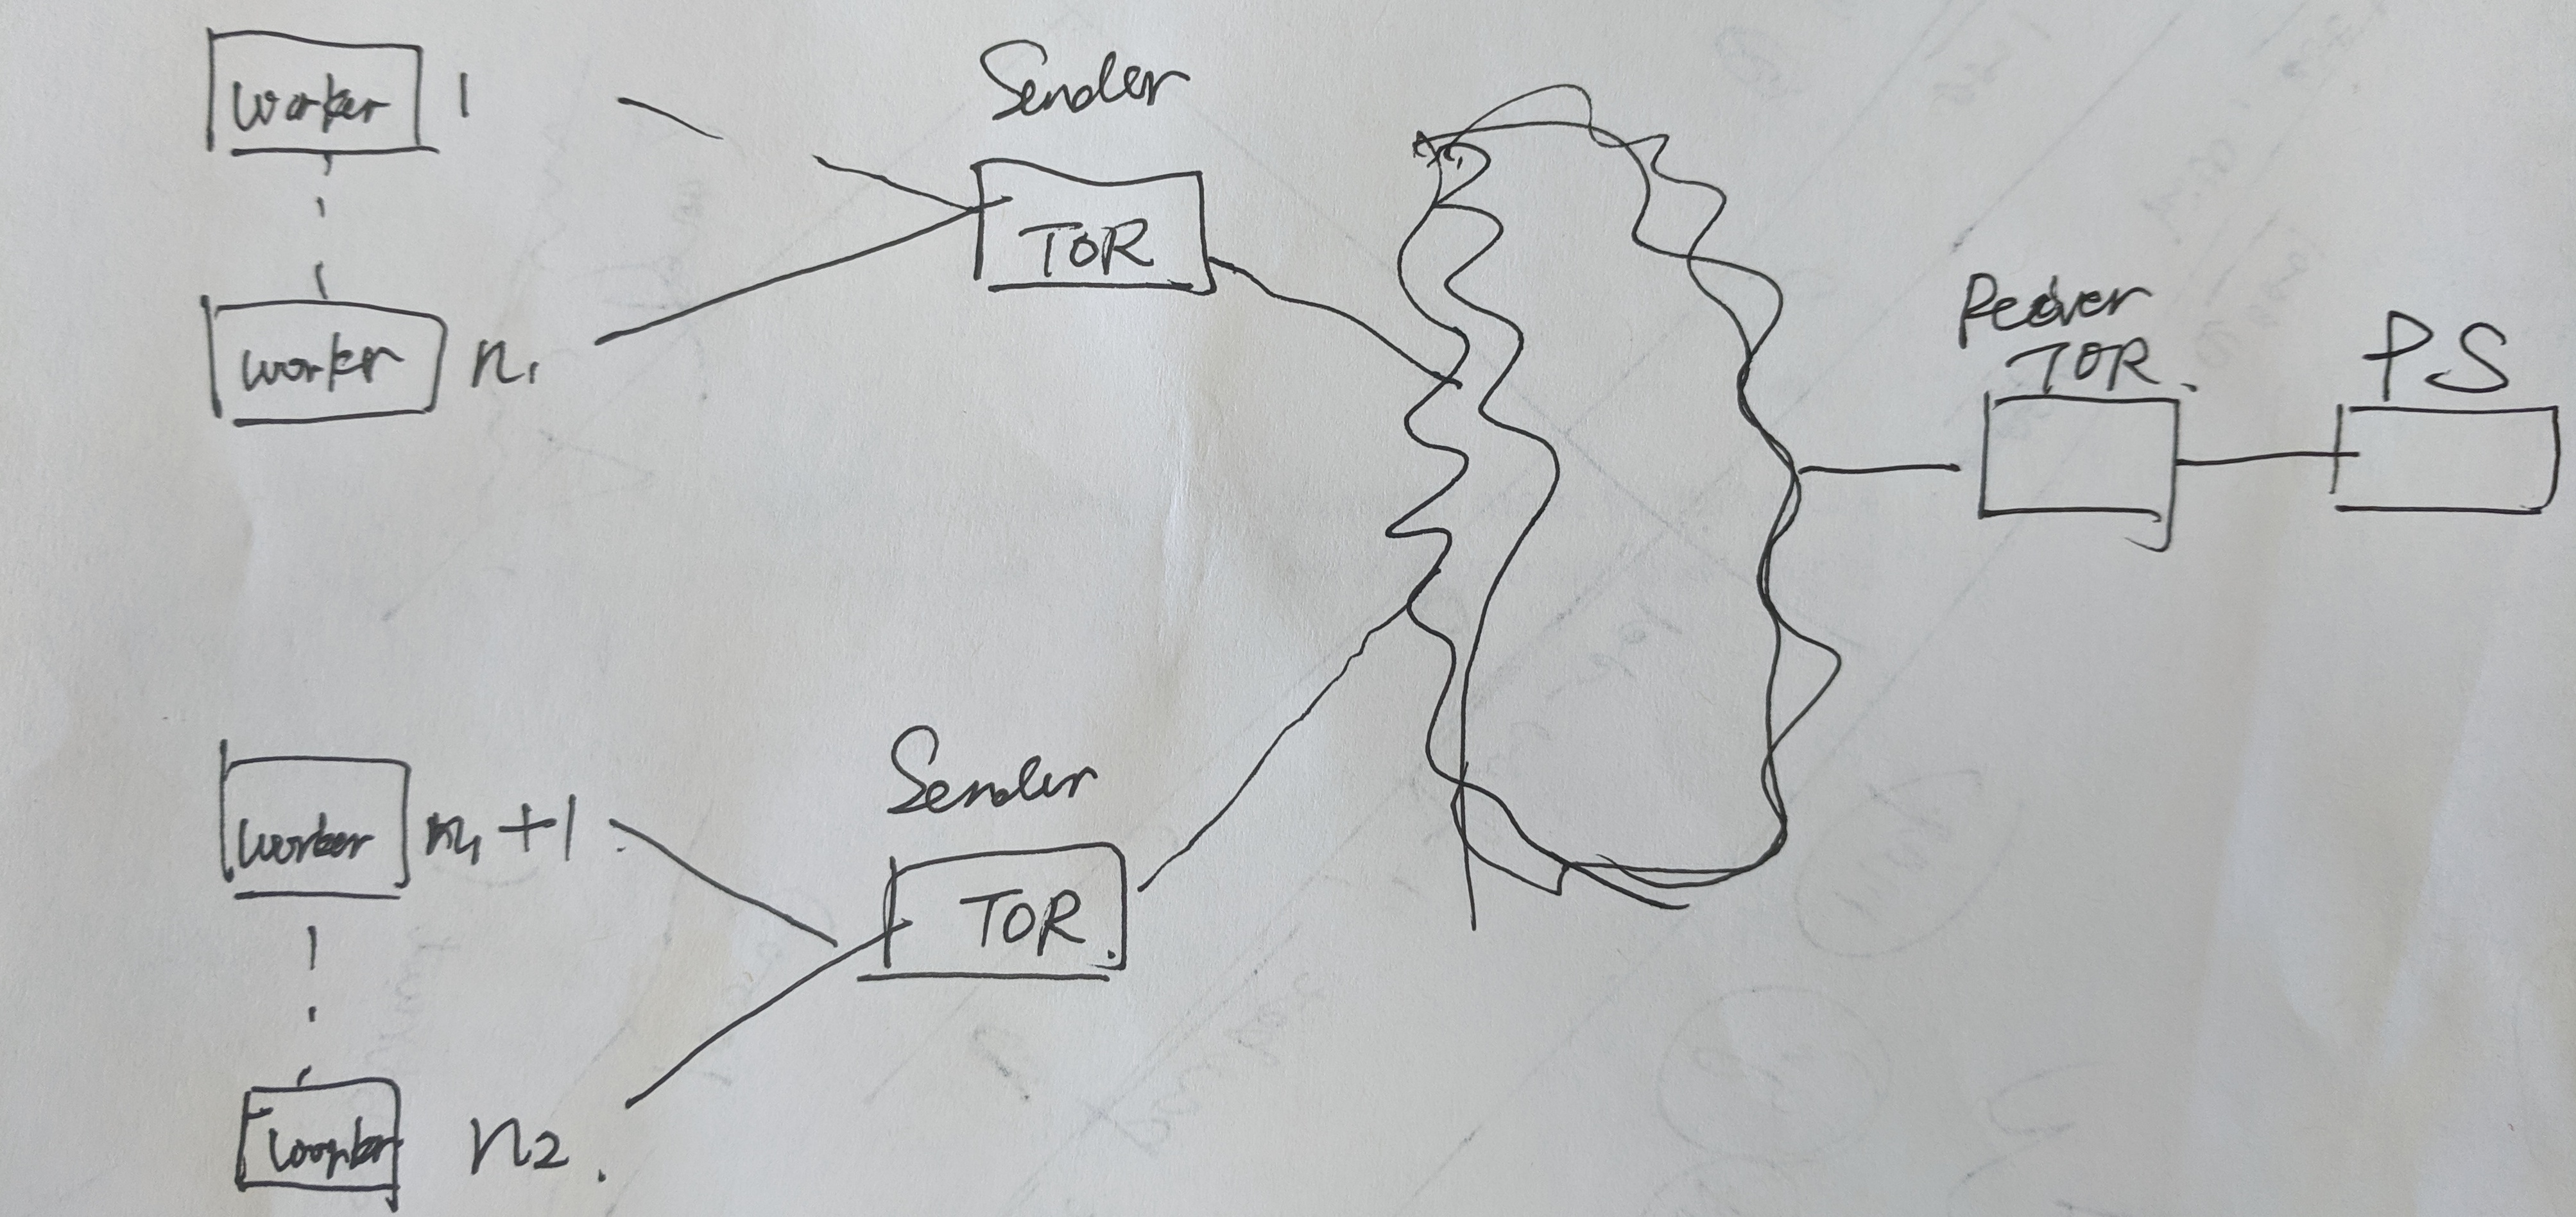
\includegraphics[width=1.0\linewidth]{figures/p4ml-arch.jpg}
    \caption{\system Architecture}
    \label{fig:p4ml-arch}
\end{figure}
\begin{figure}
    \centering
    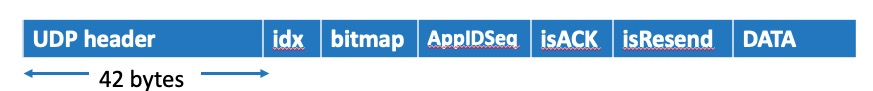
\includegraphics[width=1.0\linewidth]{figures/pktformat.jpeg}
    \caption{\system Packet Format}
    \label{fig:packet-format}
\end{figure}
\begin{table}[h!]
  \begin{center}
    \caption{Packet Fields.}
    \label{tab:packet-field}
    \begin{tabular}{|l|c|} 
	\hline
		\textbf{Field} & \textbf{Description} \\
      \hline
      idx & the aggregator position in switch.\\
      \hline
		bitmap & worker position within ToR switch. \\
      \hline
		AppIdSeq & Application ID and sequence number of a packet.\\
	  \hline
		isACK & 1, if it is the aggregation result packet, otherwise, 0. \\
		\hline
		isResend & 1, if it is a retransmitted packet, otherwise, 0. \\
		\hline 
		DATA &  128 bytes gradients value. \\
		\hline 
    \end{tabular}
  \end{center}
\end{table}
We propose \system, a in-network aggregation framework for machine learning systems.
Figure~\ref{fig:p4ml-arch} shows the architecture of \system. 
\system keeps the same architecture, workers and parameter server, as general machine learning systems
while has the aggregation functionality deployed in the ToR switches of the workers and parameter server.


In this architecture, workers do the computation, and transfer the gradients to parameter server.
via \system networking stack. The networking stack of \system packs the data into \system 
packet format, guarantees the reliability of packet delivery, and provides the congestion control
to achieve the high utilization of the link.
In addition for providing the basic switching to the traffic going through the switch, 
the switch also offers the aggregation between multiple packets and forwards the aggregation results
to the parameter server.
Finally, the parameter server receives the aggregation result, restores the aggregation results for persistency, 
and send the aggregation results after putting an ACK flag into the packet header.

The packet format is crucial for the communication between the switches and end hosts. 
We present \system packet format in Figure~\ref{fig:packet-format}, where the \system
control information is above the UDP header. The description of the fields is shown in
Table~\ref{tab:packet-field} and we will discuss how these fields are used 
to guarantee the correctness of the computation in the dataplane later in this section 
As aggregation operations are stateful operations, thus, we
need use register in the switch. The tofino switch has maximum of $12$ stages and each stages
can only process up to $4$ registers. As the control information presented in 
Table~\ref{tab:packet-field}, we finally take $8$ stages with each stage processing $4$ $32$-$bit$
integers, which results in total of $128$ bytes gradients value per packets.

\subsection{Packet I/O Efficiency}
One of the concern naturally raised from such small packets in the network is whether 
such in-network aggregation system can keep up with the line rate (i.e., 100Gbps) as CPU 
is the bottleneck for sending and receiving packets.
The state-of-the-art userspace networking programming models, e.g., RDMA, DPDK, Raw Ethernet
requires the CPUs of sender and receiver post packet descriptors to the NIC such
that NIC can do DMA read or write.

We pick the RAW Ethernet as userspace programming library. As you can see in Figure~\ref{fig:io-optimization},
without any hardware acceleration, we can only get the maximum throughput of 10Gbps in our packet IO
benchmarking with \system packet size. 
\yanfang{need a figure with 3 bars. sending/receiving packets in cpu: 10Gbps, with TSO at sender/receive in cpu: 34Gbps; with TSO at sender/mp-qp in receiver: 50Gbps.}


We find that commodity NICs, e.g., Mellanox RNICs, supports TCP Segmentation Offload~\footnote{Note it supports any packet format though the name refers to TCP packets.}, called TSO~\cite{}. TSO enables the NIC to accept 
large chunk of data with the size greater than MTU. The 
TSO engine at NIC splits the data into multiple packets with the 
user-specified packet size and inserts the user-specified headers per packet in NIC.
With TSO, CPU is released while the sending rate is increased due to this hardware offloading. 
As we can see the Figure~\ref{}, the throughput jumps to 35Gbps with TSO.

We found another advanced feature supported by the commodity NICs for the receiver side acceleration, 
called {\it multi-packet} RQ. MP-RQ can specific multiple contiguous packet buffers
using base address, buffer size, and number of buffers, which indicates the CPU can only post one packet descriptor while receiving multiple packets. With the default configuration of the $512$ packets per receive descriptor, 
\system is able to get around 50Gbps echo throughput with support of TSO and MP-RQ. 
We argue that this is the upper bound throughput per worker in a 100Gbps network in the distributed machine learning systems
as the link to the parameter servers is the bottleneck and shared by at least $2$ workers.

\begin{algorithm}[ht!]
	\caption{\textbf{Function CleanSTATE($pkt$)}}
    \begin{algorithmic}[1]
			\IF {pkt.AppIdSeqnum == AppIdSeqnum[pkt.idx] }
			\STATE agg[pkt.idx] = 0
			\STATE bitmap[pkt.idx] = 0
			\STATE AppIdSeqnum[pkt.idx] = 0
			\ENDIF
	\end{algorithmic}
    \label{func:stateclean}
    \end{algorithm}
\subsection{Strawman solution}
We begin by describing a strawman solution, which only consider the aggregation in
switch within a rack.
It assumes that (1) no packet loss; (2) the aggregator in switch is always available
whenever a packet from worker is sent to the switch;
(3) \system is the only traffic in the switch;
(4) the network is rack-scale.
We will show how the complete design of \system removes these assumptions in section~\ref{}-~\ref{}.

\subsubsection{Switch Logic}
\begin{algorithm}[ht!]
    \caption{ Switch Logic of Strawman solution}
    \begin{algorithmic}[1]
        \STATE \textbf{Initialization:}
		\STATE AppIdSeqnum[s]:={0}
		\STATE bitmap[s]:={0}
		\STATE agg[s]:= {0} 
        \vspace{4mm}
		\STATE {Extract packet fields pkt(idx, bitmap, forwarding, AppIdSeqnum, isACK, vector) }
		\IF {pkt.ACK == 0}
		\IF {AppIdSeqnum[pkt.idx] == 0}
		\STATE AppIdSeqnum[pkt.idx] = pkt.AppIdSeqnum
		\ENDIF
		\IF {pkt.AppIdSeqnum == AppIdSeqnum[pkt.idx] }
		\STATE bitmap[pkt.idx] = bitmap[pkt.idx] | pkt.bitmap
		\IF {bitmap[pkt.idx] \textbf{XOR} pkt.bitmap != 0}
		\STATE	agg[pkt.idx] = agg[pkt.idx] + pkt.vector
		\ELSE
		\STATE drop pkt
		\ENDIF
		\IF {bitmap[pkt.idx] == pkt.forwarding}
		\STATE  pkt.vector = agg[pkt.idx]
		\STATE  forward pkt to parameter server
		\ELSE
		\STATE drop pkt
        \ENDIF
		\ENDIF
		\ELSE
		\STATE CleanSTATE(pkt)
		\STATE multicast pkt
		\ENDIF
	%%	\ENDFUNCTION
	\end{algorithmic}
    \label{algo:strawman-scheduler-switch}
    \end{algorithm}
Switch has the core logic (shown in Algorithm~\ref{algo:strawman-scheduler-switch}) to provide the in-network computation.
The switch first allocates a big pool of memory when it starts and initialize 
the value as $0$ (line $4$ in Algo~\ref{algo:strawman-scheduler-switch}). This is because the switch dataplane can not 
allocate memory for the aggregation during run-time.

When a packet arrives to the switch, the 'idx' field in the packet header indicates the aggregator index at the switch.
The switch maintains a AppIdSeqnum for each packet to verify whether it is the right memory location to do the aggregation. 
Upon receiving a \system packet, the switch first check if the targeting aggregator is occupied. 
If not, it claims the usage of this aggregator (line 7-9 in Algo~\ref{algo:strawman-scheduler-switch}).
After validating that it is the right memory location to do the aggregation and check that the same packet has not been aggregated,
the switch updates the bitmap value to indicates the expected packets from this worker is done with the aggregation to guarantee
that the aggregation on the same packet happens exactly once (line 12-14 in Algo~\ref{algo:strawman-scheduler-switch}).
Finally, if the expected same sequence packets from all the workers are received, the switch writes the aggregation
results to the packet, and forward the packet to the parameter server; otherwise, it drops the packet (line 17-22 in Algo~\ref{algo:strawman-scheduler-switch}).

We use 'isACK' to indicates that this is a packet which contains the aggregation results.
The switch seeing the packet with 'isACK' set does not do aggregation, and instead 
clean all states for this packet, multicasts
this packet to all the workers (line 24-27in Algo~\ref{algo:strawman-scheduler-switch}). 
The ideal moment to clean the state should happen when the aggregation is done. However, due to 
the limitation that the same memory region can not be visited twice in Tofino switch, we push 
this action when the parameter sent the aggregation results back to the worker.

\subsubsection{Worker Logic and Parameter Server Logic}



\subsection{Challenges}
\subsection{Full utilization of switch resources}
\subsection{CC and packet loss}
\subsection{data center scale design}

\begin{algorithm}[ht!]
    \caption{\system Switch logic handling packet loss and resource sharing }
    \begin{algorithmic}[1]
        \STATE \textbf{Initialization:}
		\STATE AppIdSeqnum[s]:={0}
		\STATE bitmap[s]:={0}
		\STATE agg[s]:= {0}
        \vspace{4mm}
		\STATE {Extract packet fields pkt(idx, bitmap, forwarding, AppIdSeqnum, isACK, isResend, vector) }
		\IF {pkt.isResend == 1}
		\STATE CleanSTATE(pkt)\COMMENT{handle packet loss}
		\STATE forward pkt to parameter server
		\ELSE
		\IF {pkt.ACK == 0}
		\IF {AppIdSeqnum[pkt.idx] == 0}
		\STATE AppIdSeqnum[pkt.idx] = pkt.AppIdSeqnum
		\ENDIF
		\IF {pkt.AppIdSeqnum == AppIdSeqnum[pkt.idx]}
		\STATE bitmap[pkt.idx] = bitmap[pkt.idx] | pkt.bitmap
		\STATE	agg[pkt.idx] = agg[pkt.idx] + pkt.vector
		\IF {bitmap[pkt.idx] == pkt.forwarding}
		\STATE  pkt.vector = agg[pkt.idx]
		\STATE  forward pkt to parameter server
		\ELSE
		\STATE drop pkt
        \ENDIF
        \ELSE
		\STATE forward pkt to parameter server \COMMENT{best effort, let PS handle}
		\ENDIF
		\ELSE
		\STATE CleanSTATE(pkt)
		\STATE multicast pkt
		\ENDIF
		\ENDIF
	%%	\ENDFUNCTION
	\end{algorithmic}
    \label{algo:scheduler-switch}
    \end{algorithm}


\begin{algorithm}[ht!]
    \caption{\system Switch logic with Two level aggregation }
    \begin{algorithmic}[1]
        \STATE \textbf{Initialization:}
		\STATE AppIdSeqnum[s]:={0}
		\STATE bitmap[s]:={0}
		\STATE agg[s]:= {0}
        \vspace{4mm}
		\STATE {Extract packet fields pkt(idx, bitmap, WorkerToRforwarding, PsToRforwarding, AppIdSeqnum, isACK, isResend, vector) }
		\IF {pkt.isResend == 1}
		\STATE CleanSTATE(pkt)\COMMENT{handle packet loss}
		\STATE forward pkt to parameter server
		\ELSE
		\IF {pkt.ACK == 0}
		\IF {AppIdSeqnum[pkt.idx] == 0}
		\STATE AppIdSeqnum[pkt.idx] = pkt.AppIdSeqnum
		\ENDIF
		\IF {pkt.AppIdSeqnum == AppIdSeqnum[pkt.idx]}
		\STATE bitmap[pkt.idx] = bitmap[pkt.idx] | pkt.bitmap
		\STATE	agg[pkt.idx] = agg[pkt.idx] + pkt.vector
		\IF {bitmap[pkt.idx] == pkt.forwarding}
		\STATE  pkt.vector = agg[pkt.idx]
		\STATE  forward pkt to parameter server
		\ELSE
		\STATE drop pkt
        \ENDIF
        \ELSE
		\STATE forward pkt to parameter server \COMMENT{best effort, let PS handle}
		\ENDIF
		\ELSE
		\STATE CleanSTATE(pkt)
		\STATE multicast pkt
		\ENDIF
		\ENDIF
	%%	\ENDFUNCTION
	\end{algorithmic}
    \label{algo:scheduler-switch}
    \end{algorithm}
